%----------------------------------------------------------------------------
\chapter{Mapping}
%----------------------------------------------------------------------------
\section{Method}

This chapter decribes the process of building a separate static and a dynamic map (containing non-moving and moving obstacles, respectively) based on radial distance measurements (in this case provided by a LIDAR). Isolating the static and the moving obstacles from each other has its difficulties but also its advantages. First of all, the implemented local track planner calculates safer, more optimized paths if it is informed of both the static and the dynamic obstacles along the path. Secondly, \href{https://en.wikipedia.org/wiki/Simultaneous_localization_and_mapping}{SLAM} (Simultaneous localization and mapping) algorithms work better if the their input contains only static objects in the space, because they build an internal map of the world. Passing detections of moving obstacles to a SLAM algorithm may lead to worse localization quality, as they may ruin this map.

As a first subtask of the mapping project, I checked if any implementation is avaiable already, that can handle dynamic objects. One possible candidate was \href{http://wiki.ros.org/gmapping}{gmapping}, which is a popular ROS package, used in a wide variety of applications that require map-building and localization. Its SLAM algorithm takes LIDAR measurements as its input and generates an occupancy grid (a 2D map) of the car's environment. By using this map it is able to correct the car's (usually inaccurate odometry-based) position and orientation. I tried out the package, and the result maps were promising, the generated map was insensitive to the car's longitudinal movements and its rotations. But unfortunately, gmapping's SLAM does not support dynamic objects. The algorithm does not recognize changes in the environment, therefore if an object has been detected and placed in its map, it will not be erased from there, even after the objects has moved away. Figures \ref{gmapping_drawback_before_move} and \ref{gmapping_drawback_after_move} demonstrate the problem.

\begin{figure}[!ht]
\centering
\subfloat[Gazebo simulation]
{
    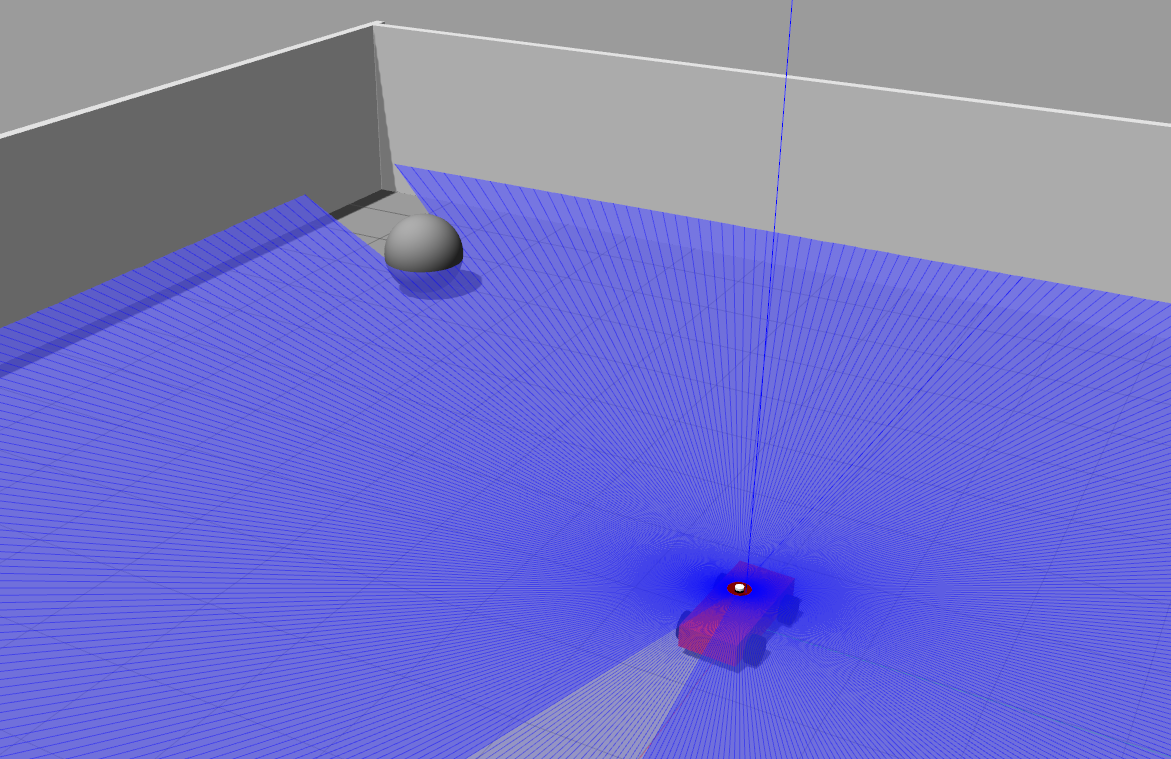
\includegraphics[height=48mm]{figures/raw/gazebo_gmapping_before_move2.png}
    \label{gazebo_gmapping_before_move}
}
\subfloat[Map created by gmapping]
{
    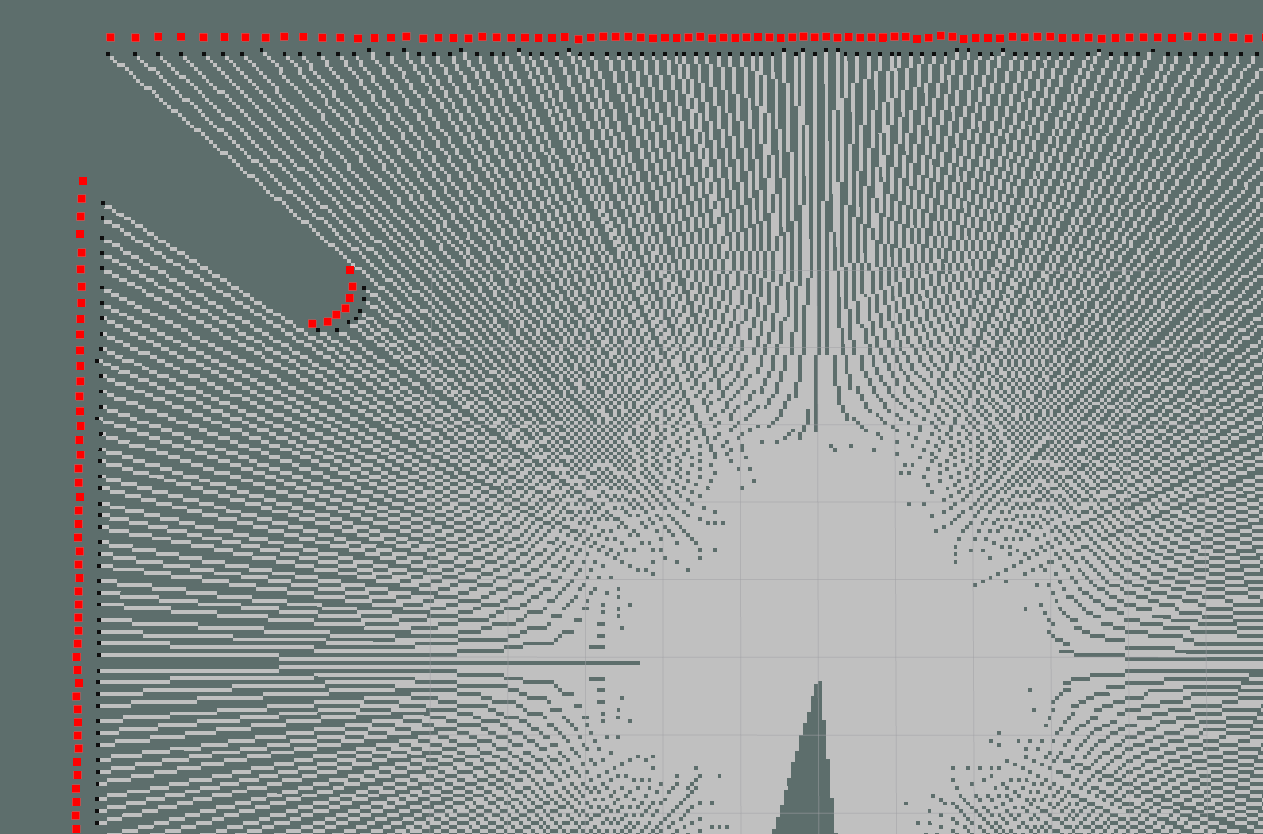
\includegraphics[height=48mm]{figures/raw/rviz_gmapping_before_move2.png}
    \label{rviz_gmapping_before_move}
}
\caption{Initial state - ball is still}
\label{gmapping_drawback_before_move}
\end{figure}

Figure \ref{gmapping_drawback_before_move} shows a situation where the ball is standing still. A the mapping algorithm of gmapping successfully creates a map (in the form of an occupancy grid) that marks the place of the ball as occupied. However, when the ball starts moving (see figure \ref{gmapping_drawback_after_move}), the map does not change, because the algorithm cannot handle moving obstacles.

\begin{figure}[!ht]
\centering
\subfloat[Gazebo simulation]
{
    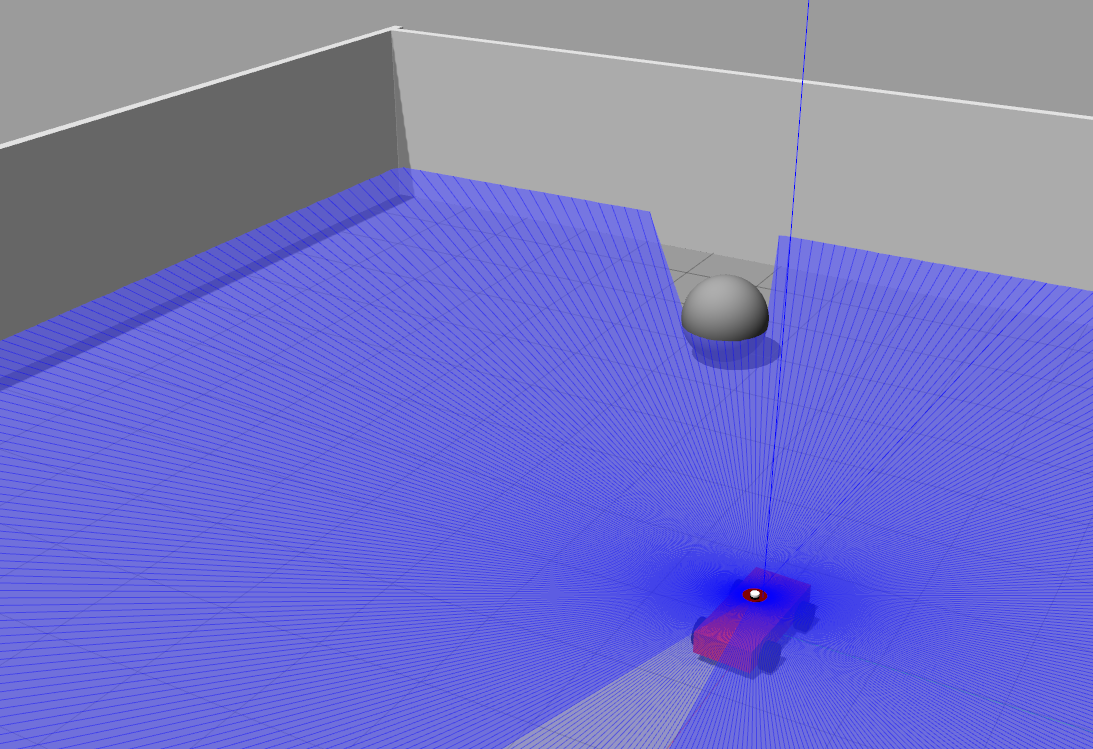
\includegraphics[height=48mm]{figures/raw/gazebo_gmapping_after_move2.png}
    \label{gazebo_gmapping_after_move}
}
\subfloat[Map created by gmapping]
{
    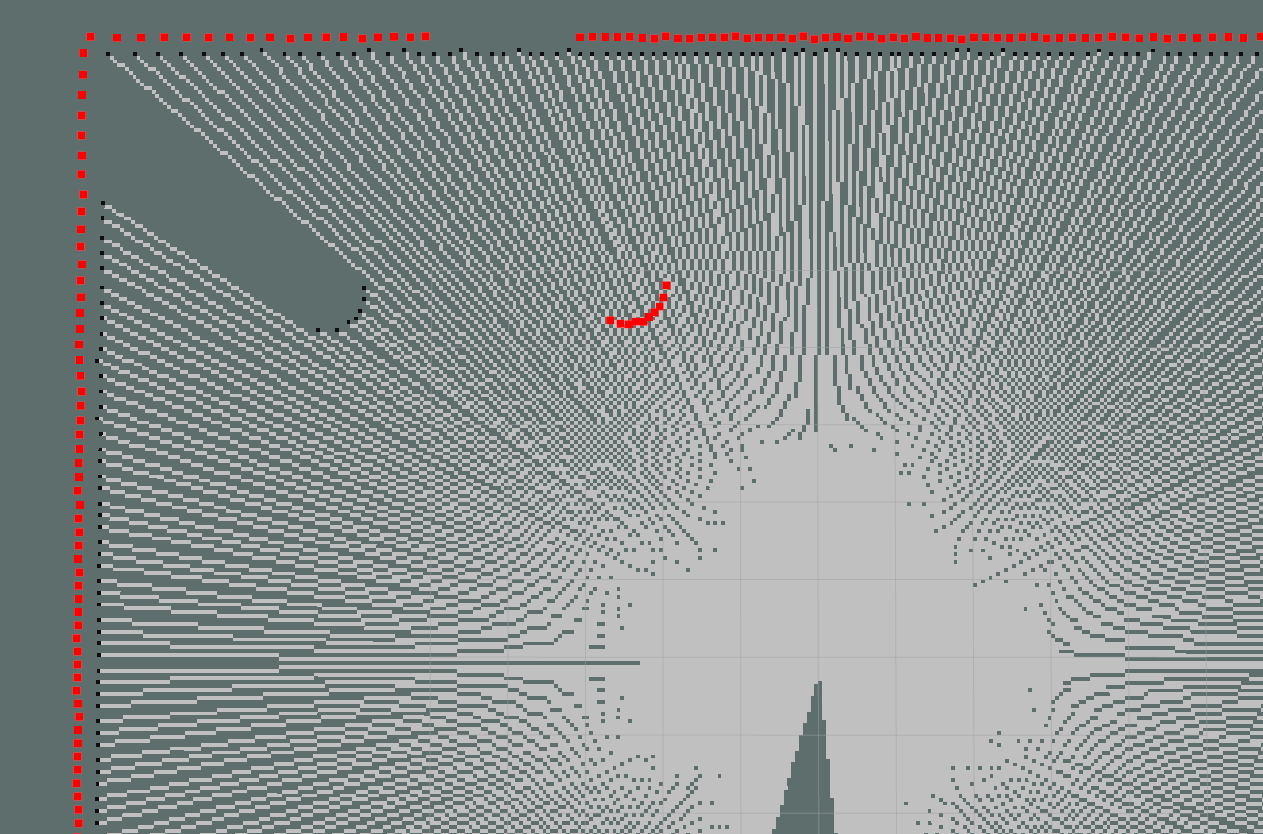
\includegraphics[height=48mm]{figures/raw/rviz_gmapping_after_move2.png}
    \label{rviz_gmapping_after_move}
}
\caption{Moving state - ball has changed position}
\label{gmapping_drawback_after_move}
\end{figure}

As a conclusion, in this project, gmapping could not be used as the producer of the static map. But that didn't mean it couln't be used for its second feature, localization. Note, that the mapping implementation I made is not a SLAM algorithm, it is not able to make corrections to the car's pose. So for that purpose, I still needed the help of gmapping, which proved to be very reliable at localization.

In order to create two disjunct maps, one static and one dynamic, the key element of the process is the separation of the moving and non-moving obstacles of the measured points.

%----------------------------------------------------------------------------
\section{Subtraction image}
%----------------------------------------------------------------------------


%----------------------------------------------------------------------------
\section{Grouping}
%----------------------------------------------------------------------------


%----------------------------------------------------------------------------
\section{Noise filtering}
%----------------------------------------------------------------------------

